\documentclass{article}
\usepackage[utf8]{inputenc}
\usepackage[a4paper, total={6in, 8.5in}]{geometry}
\usepackage{hyperref}
\usepackage{indentfirst}
\usepackage{fancyvrb}
\usepackage{array}
\usepackage{graphicx}
\usepackage{float}
\usepackage{amsmath}
\usepackage{amstext}

\usepackage{caption}
\usepackage{subcaption}

\title{Advanced programming for HPC}
\author{Minh Long PHAM - M21.ICT.008}
\date{December 2022}

\begin{document}

\maketitle

\section{Hardware}
The following hardwares were used to do the labwork:
\begin{itemize}
    \item CPU: Intel Core i5-8250U 
    \item GPU: NVIDIA GeForce MX130
\end{itemize}

\section{Implementation}
The steps to do the labwork:
\begin{itemize}
    \item Load an RGB image to an multidimensional array, which has the shape of (height, width, 3).
    \item Add padding to the image, which makes the shape of the image become (height+padding, width+padding, 3).
    \item Feed the array of image to the functions to implement Kuwahara filter using manual method with CPU and CUDA with GPU.
    \item Save images and compare the implementation time between two functions.
\end{itemize}

\begin{figure}[H]
    \center{
        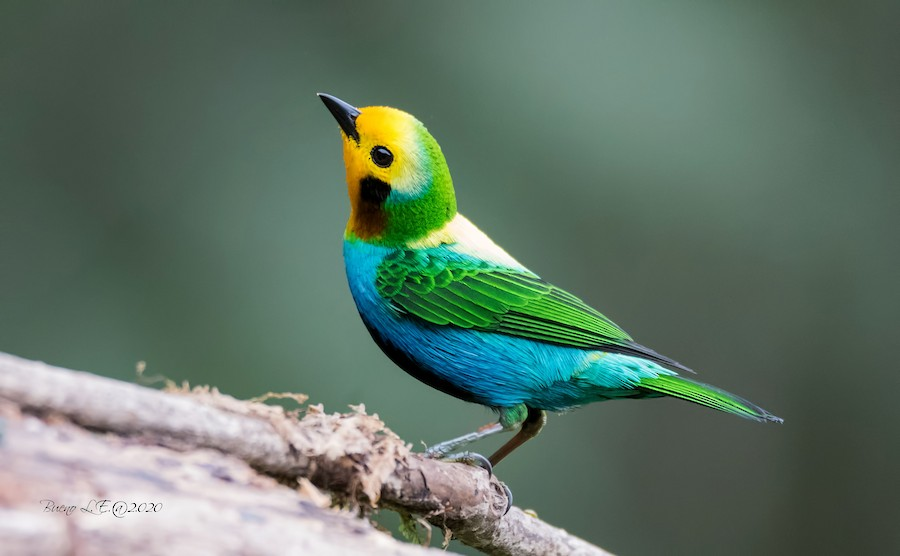
\includegraphics[scale=0.3]{images/bird.png}
    }
    \caption{Sample image}
\end{figure}

\begin{figure}[H]
    \center{
        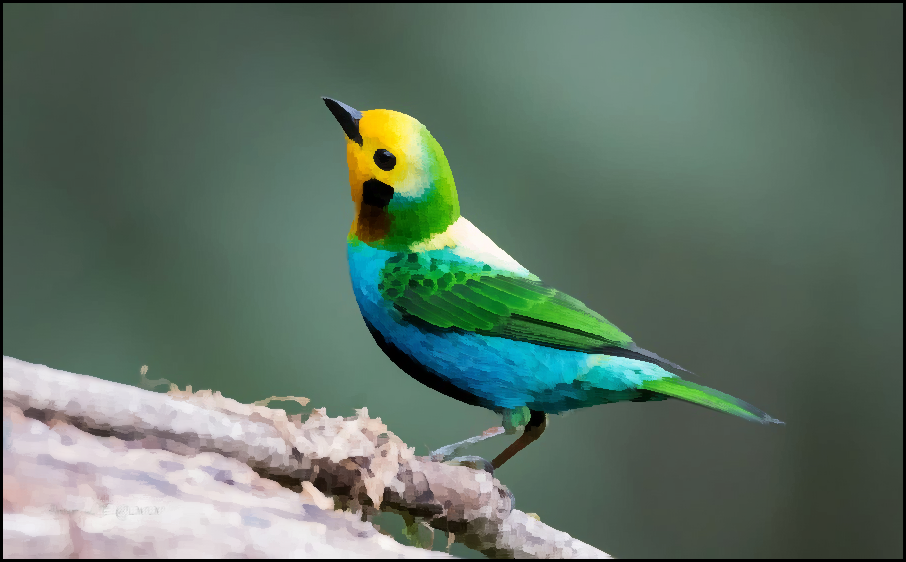
\includegraphics[scale=0.65]{images/cputransformed.png}
    }
    \caption{Implementation of Kuwahara filter using CPU}
\end{figure}

\begin{figure}[H]
    \center{
        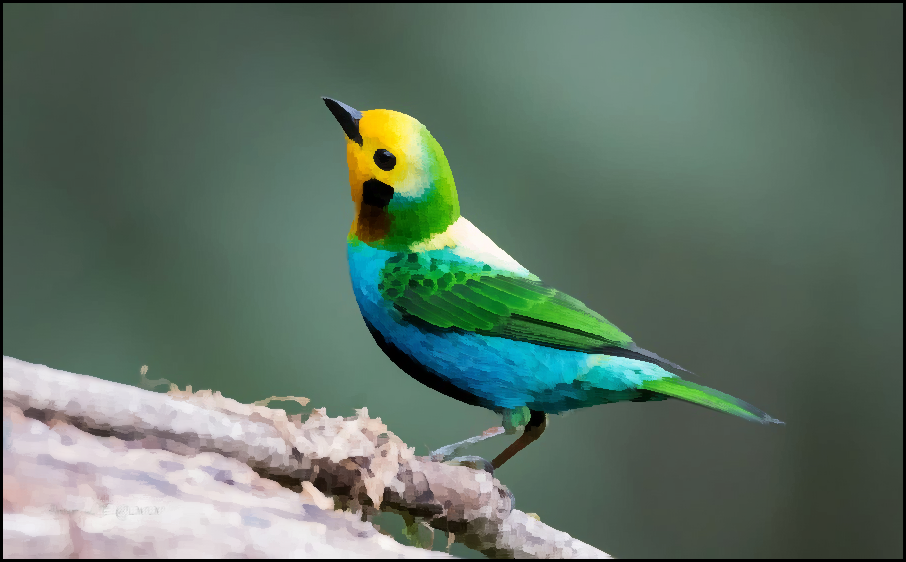
\includegraphics[scale=0.65]{images/gputransformed.png}
    }
    \caption{Implementation of Kuwahara filter using GPU}
\end{figure}

Before transforming from RGB to HSV, each value has to be scaled from [0, 255] to [0, 1]. Since I used $matplotlib.pyplot$ to load data to a numpy array, the value of each point was already in the range [0, 1] so I did not have to do much with this step. After that, I used the max and min value among Red, Green, and Blue values of each pixel to calculate the delta value which is max - min. The H, S, and V value of each pixel is calculated by the following formulae:

\begin{equation*}
  H =
    \begin{cases}
      0 & \text{if }delta = 0\\
      60 $×$ (\frac{G-B}{delta} $ mod $ 6) & \text{if }max = R\\
      60 $×$ (\frac{B-R}{delta} $+$ 2) & \text{if }max = G\\
      60 $×$ (\frac{R-G}{delta} $+$ 4) & \text{if }max = B
    \end{cases}       
\end{equation*}

\begin{equation*}
  S =
    \begin{cases}
      0 & \text{if }max=0\\
      \frac{delta}{max}
    \end{cases}       
\end{equation*}

\begin{equation*}
  V = max
\end{equation*}

It can be seen that the resultant images have a slim contour around the images, which is the padding. Other than that, the results using both CPU and GPU methods are the same. The main reason for adding padding to the image is to calculate the windows value for pixels that are on the edge of the image. 

For each pixel, I defined a list of windows' ranges to loop over it so that repetition code can be avoided. For detecting the area having the smallest standard deviation value, I declared 2 individual variable, the first one is for the index of the window having the smallest standard deviation, and the second one is the smallest standard deviation. In the beginning, I looped over the windows list to calculate thestandard deviation value for each window. If there is a smaller value of standard deviation in the loop, it will set new values for the standard deviation variable and also the index for the index variable. Since the loop is executed sequentially, I can use the index variable to retrieve the window having the smallest standard deviation value in the list of windows' range.

\begin{verbatim}
        minid = 0
        minstd = 9999.0 
        coorList = (((tidx-padsize, tidx+1), (tidy-padsize, tidy+1)),
                    ((tidx, tidx+padsize+1), (tidy-padsize, tidy+1)),
                    ((tidx-padsize, tidx+1), (tidy, tidy+padsize+1)),
                    ((tidx, tidx+padsize+1), (tidy, tidy+padsize+1)))
\end{verbatim}


Regarding the benchmark, due to the limitation of the local hardware, I can only set the block size of (4, 4) at maximum for GPU implementation. I only measured the time to execute the main function implementing Kuwahara filter. In the case in which the block size is (4, 4), the execution time using GPU was less than 1 second, which is much faster than the function to implement the filter using CPU. 

\begin{figure}[H]
    \center{
        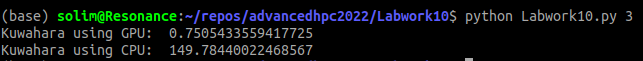
\includegraphics[scale=0.65]{images/collapsedtime.png}
    }
    \caption{Result with a block size of (4, 4)}
\end{figure}




\end{document}
